\documentclass[11pt,openany]{book}
\usepackage[]{graphicx}\usepackage[]{color}
%% maxwidth is the original width if it is less than linewidth
%% otherwise use linewidth (to make sure the graphics do not exceed the margin)
\makeatletter
\def\maxwidth{ %
  \ifdim\Gin@nat@width>\linewidth
    \linewidth
  \else
    \Gin@nat@width
  \fi
}
\makeatother

\definecolor{fgcolor}{rgb}{0.345, 0.345, 0.345}
\newcommand{\hlnum}[1]{\textcolor[rgb]{0.686,0.059,0.569}{#1}}%
\newcommand{\hlstr}[1]{\textcolor[rgb]{0.192,0.494,0.8}{#1}}%
\newcommand{\hlcom}[1]{\textcolor[rgb]{0.678,0.584,0.686}{\textit{#1}}}%
\newcommand{\hlopt}[1]{\textcolor[rgb]{0,0,0}{#1}}%
\newcommand{\hlstd}[1]{\textcolor[rgb]{0.345,0.345,0.345}{#1}}%
\newcommand{\hlkwa}[1]{\textcolor[rgb]{0.161,0.373,0.58}{\textbf{#1}}}%
\newcommand{\hlkwb}[1]{\textcolor[rgb]{0.69,0.353,0.396}{#1}}%
\newcommand{\hlkwc}[1]{\textcolor[rgb]{0.333,0.667,0.333}{#1}}%
\newcommand{\hlkwd}[1]{\textcolor[rgb]{0.737,0.353,0.396}{\textbf{#1}}}%
\let\hlipl\hlkwb

\usepackage{framed}
\makeatletter
\newenvironment{kframe}{%
 \def\at@end@of@kframe{}%
 \ifinner\ifhmode%
  \def\at@end@of@kframe{\end{minipage}}%
  \begin{minipage}{\columnwidth}%
 \fi\fi%
 \def\FrameCommand##1{\hskip\@totalleftmargin \hskip-\fboxsep
 \colorbox{shadecolor}{##1}\hskip-\fboxsep
     % There is no \\@totalrightmargin, so:
     \hskip-\linewidth \hskip-\@totalleftmargin \hskip\columnwidth}%
 \MakeFramed {\advance\hsize-\width
   \@totalleftmargin\z@ \linewidth\hsize
   \@setminipage}}%
 {\par\unskip\endMakeFramed%
 \at@end@of@kframe}
\makeatother

\definecolor{shadecolor}{rgb}{.97, .97, .97}
\definecolor{messagecolor}{rgb}{0, 0, 0}
\definecolor{warningcolor}{rgb}{1, 0, 1}
\definecolor{errorcolor}{rgb}{1, 0, 0}
\newenvironment{knitrout}{}{} % an empty environment to be redefined in TeX

\usepackage{alltt}
\newcommand{\SweaveOpts}[1]{}  % do not interfere with LaTeX
\newcommand{\SweaveInput}[1]{} % because they are not real TeX commands
\newcommand{\Sexpr}[1]{}       % will only be parsed by R


\usepackage[utf8]{inputenc} 
\usepackage{amssymb, amsmath, amsthm}
\usepackage{fullpage}
\usepackage{setspace}
\usepackage{graphicx}
\usepackage{natbib}
\usepackage{rotating}
\usepackage{caption}
\usepackage{subcaption}
\usepackage{multirow}
\usepackage{booktabs}
\usepackage{dcolumn}
\usepackage[grey]{quotchap}
\usepackage{xcolor}
\usepackage[left=1in, top=1in, right=1.5in, bottom=1in, headsep=.5in]
{geometry}
\usepackage{fancyhdr, blindtext}
\usepackage{diagbox}
\usepackage{hyperref} 
\usepackage{placeins}
\renewenvironment{knitrout}{\begin{singlespace}}{\end{singlespace}}
\newcommand*{\mybox}[2]{\colorbox{#1!30}{\parbox{.98\linewidth}{#2}}}
\newcommand*{\befehl}[1]{\texttt{\textbackslash #1}} % Added by 


\fancyhf{}
\fancyhead[LE]{\slshape \rightmark} 
\fancyhead[RE]{\thepage}
\fancyhead[RO]{\slshape \leftmark} 
\fancyhead[LO]{\thepage}
\renewcommand{\headrulewidth}{0.4pt}
\pagestyle{fancy}
%% new command for greybox
\long\def\greybox#1{%
    \newbox\contentbox%
    \newbox\bkgdbox%
    \setbox\contentbox\hbox to \hsize{%
        \vtop{
            \kern\columnsep
            \hbox to \hsize{%
                \kern\columnsep%
                \advance\hsize by -2\columnsep%
                \setlength{\textwidth}{\hsize}%
                \vbox{
                    \parskip=\baselineskip
                    \parindent=0bp
                    #1
                }%
                \kern\columnsep%
            }%
            \kern\columnsep%
        }%
    }%
    \setbox\bkgdbox\vbox{
        \pdfliteral{0.85 0.85 0.85 rg}
        \hrule width  \wd\contentbox %
               height \ht\contentbox %
               depth  \dp\contentbox
        \pdfliteral{0 0 0 rg}
    }%
    \wd\bkgdbox=0bp%
    \vbox{\hbox to \hsize{\box\bkgdbox\box\contentbox}}%
    \vskip\baselineskip%
}
%% make greybox (grbox) a float
\usepackage{float}
\newfloat{grbox}{thp}{lop}[section]
\floatname{grbox}{Grey Box}



\begin{document}






\chapter{Logit Regression} 


Logit regression is a part of a larger class of generalized linear models (GLM).   In this chapter we first briefly discuss GLMs, and then move on into a more in-depth discussion of logistic regression. Once again, the examples in this chapter use the \texttt{tbur} data set. 

\section{Generalized Linear Models} 

GLMs provide a modeling structure that can relate a linear model to response variables that do not have normal distributions. The distribution of $Y$ is assumed to belong to one of an exponential family of distributions, including the Gaussian, Binomial, and Poisson distributions.  GLMs are fit to the data by the method of maximum likelihood. 

Like OLS, GLMs contain a stochastic component and a systematic component. The systematic component is expressed as: 
\begin{equation}
  \eta = \alpha + \beta_1 X_{i1} + \beta_2 X_{i2} + \ldots + \beta_k X_{ik}
\end{equation}
However, GLMs also contain a ``link function" that relates the response variable, $Y_i$, to the systematic linear component, $\eta$.  Table 16.1 shows the major exponential “families” of GLM models, and indicates the kinds of link functions involved in each.  Note that OLS models would fall within the Gaussian family.  In the next section we focus on the binomial family, and on logit estimation in particular.

\begin{figure}
        \centering
        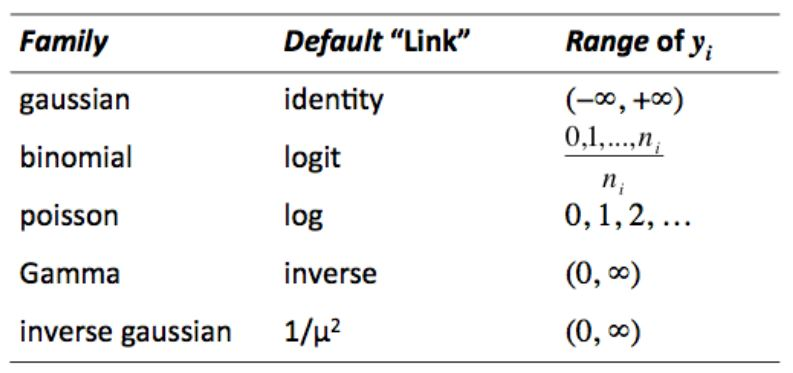
\includegraphics[width=4in]{../16_Logit/families.jpg}%filename
        \caption{Exponential ``families" of GLM Models}
\end{figure} 
 

\section{Logit Estimation} 

Logit is used when predicting limited dependent variables,
specifically those in which $Y$ is represented by $0$’s and $1$’s.
By virtue of the binary dependent variable, these models do not meet the
key assumptions of OLS. Logit uses maximum likelihood estimation (MLE),
which is a counterpart to minimizing least squares. 
MLE identifies the probability of obtaining the sample as a function
of the model parameters (i.e., the $X$’s). It answers the question, 
what are the values for $B$’s that make the sample most likely? In
other words, the likelihood 
function expresses the probability of obtaining the observed data as a
function of the model parameters. Estimates of $A$ and $B$ are based
on maximizing a likelihood function of the observed $Y$ values.  
In logit estimation we seek $P(Y=1)$, the probability that $Y=1$. The
odds that $Y=1$ is expressed as:

\begin{equation*}
  O(Y=1)=\frac{P(Y=1)}{1-P(Y=1)}
\end{equation*}

\noindent Logits, $L$, are the natural logarithm of the odds: 

\begin{align*}
  L &= log_e O \\
  &=log_e \frac{P}{1-P}
\end{align*}

\noindent They can range from $-\infty$, when $P=0$, to $\infty$, when
$P=1$. $L$ is the estimated systematic linear component: 

\begin{equation*}
  L = A+B_1 X_{i1}+\ldots+B_k X_{ik}
\end{equation*}

\noindent By reversing the logit we can obtain the predicted
probability that $Y=1$ for each of the $i$ observations. 

\begin{equation}
  \label{eq:predprob}
  P_{i} = \frac{1}{1-e^{-L_{i}}}
\end{equation}

\noindent where $e=2.71828 \ldots$, the base number of natural
logarithms. Note that $L$ is a linear function, but $P$ is a non-linear
$S$-shaped function as shown in Figure \ref{fig:logex}. Also note,
that Equation 16.2 is the link function that relates the
linear component to the non-linear response variable.  
%  removed this and did a hard code; could not figure out the problem.
%  \ref{eq:predprob}

\begin{figure}
        \centering
        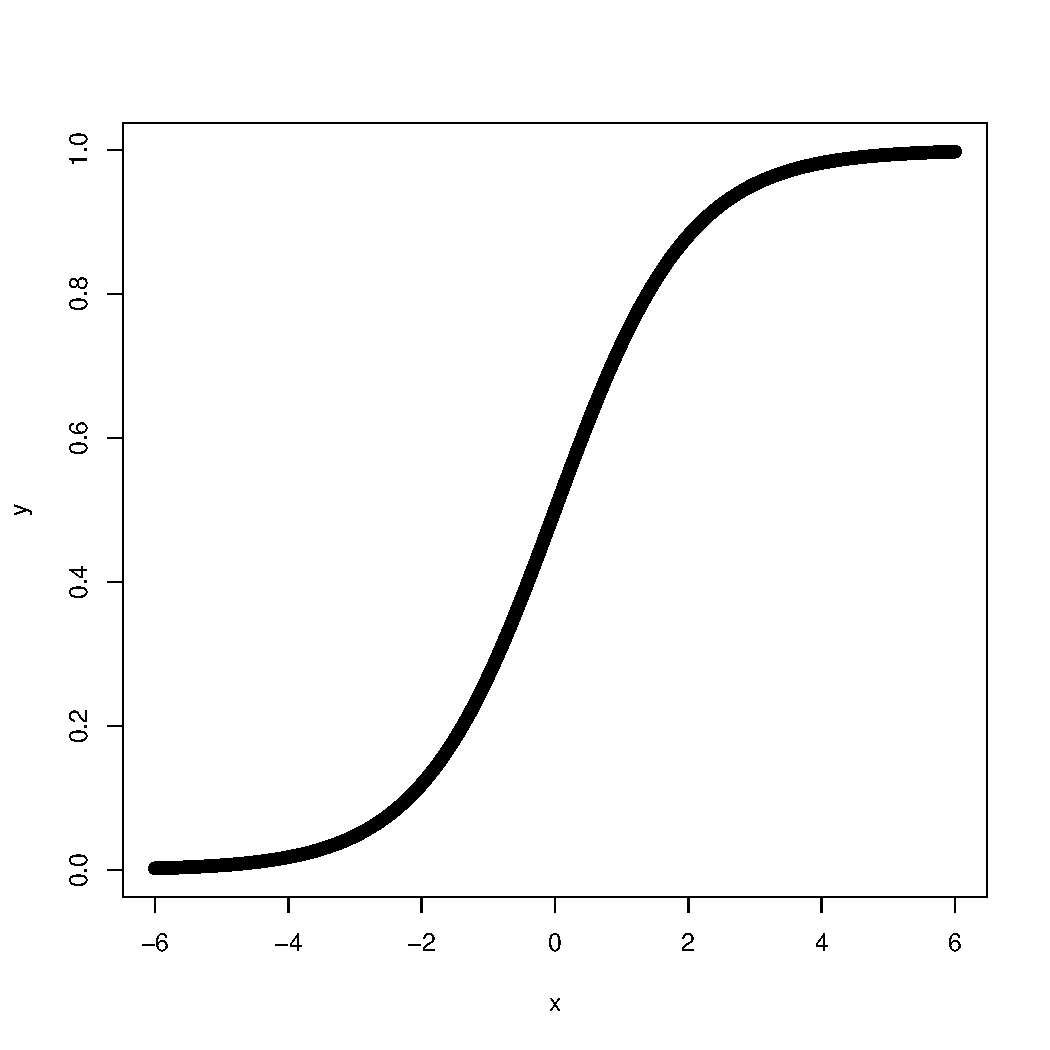
\includegraphics[width=4in]{../16_Logit/logex.pdf}%filename
        \caption{Predicted Probability as a Logit Function of $X$ \label{fig:logex}}
\end{figure}   

In more formal terms, each observation, $i$,  contributes to the likelihood function by $P_i$ if $Y_i=1$, and by $1-P_i$ if $Y_i=0$. This is defined as: 
\begin{equation*}
  P^{Y_{i}}_i(1-P_i)^{1-Y_i}
\end{equation*}
\noindent The likelihood function is the product (multiplication) of all these individual contributions:
\begin{equation*}
  \ell = \prod P^{Y_{i}}_i(1-P_i)^{1-Y_i}
\end{equation*}
\noindent The likelihood function is the largest for the model that best predicts $Y=1$ or $Y=0$, therefore when the predicted value of $Y$ is correct and close to $1$ or $0$, the likelihood function is maximized. 

To estimate the model parameters, we seek to maximize the log of the likelihood function. We use the log because it converts the multiplication into addition, and is therefore easier to calculate. The log likelihood is:
\begin{equation*}
  \text{log}_e \ell = \sum^{n}_{i=1}[Y_i \text{log}_e P_i+(1-Y_i)\text{log}_e(1-P_i)]
\end{equation*}

The solution involves taking the first derivative of the log likelihood with respect to each of the $B$’s, setting them to zero, and solving the simultaneous equation.  The solution of the equation isn't linear, so it can't be solved directly.  Instead, it's solved through a sequential estimation process that looks for successively better ``fits'' of the model. 

For the most part, the key assumptions required for logit models are analogous to those required for OLS. The key differences are that (a) we do not assume a linear relationship between the $X$s and $Y$, and (b) we do not assume normally distributed, homoscedastistic residuals. The key assumptions that are retained are shown below.

\begin{grbox}
\greybox{\textbf{Logit Assumptions and Qualifiers}   
\begin{itemize}
\item The model is correctly specified
\begin{itemize}
\item True conditional probabilities are logistic function of the $X$’s
\item No important $X$’s omitted; no extraneous $X$’s included
\item No significant measurement error
\end{itemize}  
\item The cases are independent
\item No $X$ is a linear function of other $X$’s
\begin{itemize}
\item Increased multicollinearity leads to greater imprecision
\end{itemize}
\item Influential cases can bias estimates
\item Sample size: $n-k-1$ should exceed $100$ 
  \begin{itemize}
\item Independent covariation between the $X$s and $Y$ is critical
  \end{itemize}
  \end{itemize}}
\end{grbox}

 
The following example uses demographic information to predict beliefs about anthropogenic climate change. 



\begin{knitrout}
\definecolor{shadecolor}{rgb}{0.969, 0.969, 0.969}\color{fgcolor}\begin{kframe}
\begin{alltt}
\hlstd{logit1} \hlkwb{<-} \hlkwd{glm}\hlstd{(glbcc} \hlopt{~} \hlstd{age} \hlopt{+} \hlstd{gender} \hlopt{+} \hlstd{education} \hlopt{+} \hlstd{income,} \hlkwc{data} \hlstd{= ds.temp,} \hlkwc{family} \hlstd{=} \hlkwd{binomial}\hlstd{())}
\hlkwd{summary}\hlstd{(logit1)}
\end{alltt}
\begin{verbatim}
## 
## Call:
## glm(formula = glbcc ~ age + gender + education + income, family = binomial(), 
##     data = ds.temp)
## 
## Deviance Residuals: 
##    Min      1Q  Median      3Q     Max  
## -1.707  -1.250   0.880   1.053   1.578  
## 
## Coefficients:
##               Estimate Std. Error z value Pr(>|z|)    
## (Intercept)  4.432e-01  2.344e-01   1.891 0.058689 .  
## age         -1.079e-02  3.116e-03  -3.462 0.000535 ***
## gender      -3.131e-01  8.804e-02  -3.557 0.000375 ***
## education    1.580e-01  2.513e-02   6.288 3.22e-10 ***
## income      -2.380e-06  8.013e-07  -2.970 0.002977 ** 
## ---
## Signif. codes:  0 '***' 0.001 '**' 0.01 '*' 0.05 '.' 0.1 ' ' 1
## 
## (Dispersion parameter for binomial family taken to be 1)
## 
##     Null deviance: 3114.5  on 2281  degrees of freedom
## Residual deviance: 3047.4  on 2277  degrees of freedom
## AIC: 3057.4
## 
## Number of Fisher Scoring iterations: 4
\end{verbatim}
\end{kframe}
\end{knitrout}
\noindent As we can see age and gender are both negative and statistically significant predictors of climate change opinion. Below we discuss logit hypothesis tests, goodness of fit, and how to interpret the logit coefficients.  

\subsection{Logit Hypothesis Tests} 

In some ways, hypothesis testing with logit is quite similar to that using OLS. The same use of  $p$-values is employed, however they differ in
how they are derived. The logit analysis makes use of the Wald $z$-statistic, which is similar to the $t$-stat in OLS. The Wald $z$ score compares the estimated coefficient to the asymptotic standard error, (aka the normal distribution). The $p$-value is derived from the asymptotic standard-normal distribution. Each estimated coefficient has a Wald $z$-score and a $p$-value that shows the probability that the null hypothesis is correct, given the data. 
\begin{equation}
  \label{eq:wald}
  z = \frac{B_j}{SE(B_j)} 
\end{equation}
 
\subsection{Goodness of Fit} 

Given that logit regression is estimated using MLE, the goodness-of-fit statistics differ from those of OLS. Here we examine three
measures of fit: log-likelihood, the pseudo $R^2$, and the Akaike information criteria (AIC). 

\subsubsection{Log-Likelihood}
To test for the overall null hypothesis that all $B$’s are equal to zero, similar to an overall $F$-test in OLS, we can compare the log-likelihood of the demographic model with 4 IVs to the initial ``null model" which includes only the intercept term. In general, a smaller log-likelihood indicates a better fit. Using the deviance statistic $G^2$ (aka the likelihood-ratio test statistic), we can determine whether the difference
is statistically significant. $G^2$ is expressed as: 

 \begin{equation}
   \label{eq:G}
   G^2 = 2(\text{log}_e L_1 - \text{log}_e L_0)
\end{equation}

\noindent where $L_1$ is the demographic model and $L_0$ is the null model. The $G^2$ test statistic takes the difference between the log likelihoods of the two models and compares that to a $\chi^2$ distribution with $q$ degrees of freedom, where $q$ is the difference in the number of IVs. We can calculate this in \texttt{R}.  First, we run a null model predicting belief that greenhouse gases are causing the climate to change, using only
the intercept:

\begin{knitrout}
\definecolor{shadecolor}{rgb}{0.969, 0.969, 0.969}\color{fgcolor}\begin{kframe}
\begin{alltt}
\hlstd{logit0} \hlkwb{<-} \hlkwd{glm}\hlstd{(glbcc} \hlopt{~} \hlnum{1}\hlstd{,} \hlkwc{data} \hlstd{= ds.temp)}
\hlkwd{summary}\hlstd{(logit0)}
\end{alltt}
\begin{verbatim}
## 
## Call:
## glm(formula = glbcc ~ 1, data = ds.temp)
## 
## Deviance Residuals: 
##     Min       1Q   Median       3Q      Max  
## -0.5732  -0.5732   0.4268   0.4268   0.4268  
## 
## Coefficients:
##             Estimate Std. Error t value Pr(>|t|)    
## (Intercept)  0.57318    0.01036   55.35   <2e-16 ***
## ---
## Signif. codes:  0 '***' 0.001 '**' 0.01 '*' 0.05 '.' 0.1 ' ' 1
## 
## (Dispersion parameter for gaussian family taken to be 0.2447517)
## 
##     Null deviance: 558.28  on 2281  degrees of freedom
## Residual deviance: 558.28  on 2281  degrees of freedom
## AIC: 3267.1
## 
## Number of Fisher Scoring iterations: 2
\end{verbatim}
\end{kframe}
\end{knitrout}

We then calculate the log likelihood for the null model, 
\begin{equation}\text{log}_e L_0\end{equation}

\begin{knitrout}
\definecolor{shadecolor}{rgb}{0.969, 0.969, 0.969}\color{fgcolor}\begin{kframe}
\begin{alltt}
\hlkwd{logLik}\hlstd{(logit0)}
\end{alltt}
\begin{verbatim}
## 'log Lik.' -1631.548 (df=2)
\end{verbatim}
\end{kframe}
\end{knitrout}

Next, we calculate the log likelihood for the demographic model, 

\begin{equation}\text{log}_e L_0\end{equation}

Recall that we generated this model (dubbed ``logit1") earlier:

\begin{knitrout}
\definecolor{shadecolor}{rgb}{0.969, 0.969, 0.969}\color{fgcolor}\begin{kframe}
\begin{alltt}
\hlkwd{logLik}\hlstd{(logit1)}
\end{alltt}
\begin{verbatim}
## 'log Lik.' -1523.724 (df=5)
\end{verbatim}
\end{kframe}
\end{knitrout}

Finally, we calculate the  $G$ statistic and perform the chi-square test for statistical significance:

\begin{knitrout}
\definecolor{shadecolor}{rgb}{0.969, 0.969, 0.969}\color{fgcolor}\begin{kframe}
\begin{alltt}
\hlstd{G} \hlkwb{<-} \hlnum{2}\hlopt{*}\hlstd{(}\hlopt{-}\hlnum{1523} \hlopt{-} \hlstd{(}\hlopt{-}\hlnum{1631}\hlstd{))}
\hlstd{G}
\end{alltt}
\begin{verbatim}
## [1] 216
\end{verbatim}
\begin{alltt}
\hlkwd{pchisq}\hlstd{(G,} \hlkwc{df} \hlstd{=} \hlnum{3}\hlstd{,} \hlkwc{lower.tail} \hlstd{=} \hlnum{FALSE}\hlstd{)}
\end{alltt}
\begin{verbatim}
## [1] 1.470144e-46
\end{verbatim}
\end{kframe}
\end{knitrout}

\noindent We can see by the very low p-value that the demographic model offers a significant improvement in fit. 

The same approach can be used to compare nested models, similar to nested $F$-tests in OLS. For example, we can include ideology in the model and use the \texttt{anova} function to see if the ideology variable improves model fit. Note that we specify the $\chi^2$ test. 
\begin{knitrout}
\definecolor{shadecolor}{rgb}{0.969, 0.969, 0.969}\color{fgcolor}\begin{kframe}
\begin{alltt}
\hlstd{logit2} \hlkwb{<-} \hlkwd{glm}\hlstd{(glbcc} \hlopt{~} \hlstd{age} \hlopt{+} \hlstd{gender} \hlopt{+} \hlstd{education} \hlopt{+} \hlstd{income} \hlopt{+} \hlstd{ideol,} \hlkwc{family} \hlstd{=} \hlkwd{binomial}\hlstd{(),}
    \hlkwc{data} \hlstd{= ds.temp)}
\hlkwd{summary}\hlstd{(logit2)}
\end{alltt}
\begin{verbatim}
## 
## Call:
## glm(formula = glbcc ~ age + gender + education + income + ideol, 
##     family = binomial(), data = ds.temp)
## 
## Deviance Residuals: 
##     Min       1Q   Median       3Q      Max  
## -2.6661  -0.8939   0.3427   0.8324   2.0212  
## 
## Coefficients:
##               Estimate Std. Error z value Pr(>|z|)    
## (Intercept)  4.055e+00  3.211e-01  12.629  < 2e-16 ***
## age         -4.287e-03  3.630e-03  -1.181 0.237701    
## gender      -2.044e-01  1.023e-01  -1.998 0.045702 *  
## education    1.009e-01  2.934e-02   3.440 0.000582 ***
## income      -1.042e-06  8.939e-07  -1.166 0.243485    
## ideol       -7.900e-01  3.763e-02 -20.993  < 2e-16 ***
## ---
## Signif. codes:  0 '***' 0.001 '**' 0.01 '*' 0.05 '.' 0.1 ' ' 1
## 
## (Dispersion parameter for binomial family taken to be 1)
## 
##     Null deviance: 3114.5  on 2281  degrees of freedom
## Residual deviance: 2404.0  on 2276  degrees of freedom
## AIC: 2416
## 
## Number of Fisher Scoring iterations: 4
\end{verbatim}
\begin{alltt}
\hlkwd{anova}\hlstd{(logit1, logit2,} \hlkwc{test} \hlstd{=} \hlstr{"Chisq"}\hlstd{)}
\end{alltt}
\begin{verbatim}
## Analysis of Deviance Table
## 
## Model 1: glbcc ~ age + gender + education + income
## Model 2: glbcc ~ age + gender + education + income + ideol
##   Resid. Df Resid. Dev Df Deviance  Pr(>Chi)    
## 1      2277     3047.4                          
## 2      2276     2404.0  1   643.45 < 2.2e-16 ***
## ---
## Signif. codes:  0 '***' 0.001 '**' 0.01 '*' 0.05 '.' 0.1 ' ' 1
\end{verbatim}
\end{kframe}
\end{knitrout}
\noindent As we can see, adding ideology significantly improves the model. 

\subsubsection{Pseudo $R^2$}

A measure that is equivalent to the $R^2$ in OLS does not exist for logit. Remember that explaining variance in $Y$ is not the goal of MLE. However, a ``pseudo'' $R^2$ measure exists that compares the residual deviance of the null model with that of the  full model. Like the $R^2$ measure, pseudo $R^2$ ranges from $0$ to $1$ with values closer to $1$ indicating improved model fit. 

Deviance is analogous to the residual sum of squares for a linear model. It is expressed as:

\begin{equation}
  \label{eq:dev}
  \text{deviance} = -2(\text{log}_e L)
\end{equation}

\noindent It is simply the log-likelihood of the model multiplied by a $-2$. The pseudo $R^2$ is $1$ minus the ratio of the deviance of the full model $L_1$ to the deviance of the null model $L_0$:

\begin{equation}
  \label{eq:psR2}
  \text{pseudo} R^2 = 1-\frac{-2(\text{log}_e L_1)}{-2(\text{log}_e L_0)} 
\end{equation}
\noindent This can be calculated in \texttt{R} using the full
model with ideology. 
\begin{knitrout}
\definecolor{shadecolor}{rgb}{0.969, 0.969, 0.969}\color{fgcolor}\begin{kframe}
\begin{alltt}
\hlstd{pseudoR2} \hlkwb{<-} \hlnum{1} \hlopt{-} \hlstd{(logit2}\hlopt{$}\hlstd{deviance}\hlopt{/}\hlstd{logit2}\hlopt{$}\hlstd{null.deviance)}
\hlstd{pseudoR2}
\end{alltt}
\begin{verbatim}
## [1] 0.2281165
\end{verbatim}
\end{kframe}
\end{knitrout}
\noindent The pseudo $R^2$ of the model is 0.2281165. Note that the 0.2281165 is only an approximation of explained variance, and should be used in combination with other measures of fit such as AIC.

\subsubsection{Akaike Information Criteria}
Another way to examine goodness-of-fit is the Akaike information criteria (AIC). Like the adjusted $R^2$ for OLS, the AIC takes into account the parsimony of the model by penalizing for the number of parameters. But AIC is useful only in a comparative manner -- either with the null model or an alternative model. It does not purport to describe the percent of variance in $Y$ accounted for, as does the pseudo $R^2$.

AIC is defined as -2 times the residual deviance of the model plus two times the number of parameters; $k$ IVs plus the intercept:

\begin{equation}
  \label{eq:aic}
  \text{AIC} = -2(\text{log}_e L) + 2(k+1) 
\end{equation}

\noindent Note that smaller values are indicative of a better fit. The AIC is most useful when comparing the fit of alternative (not necessarily nested) models. In $R$, AIC is given as part of the \texttt{summary} output for a \texttt{glm} object, but we can also calculate it and verify. 

\begin{knitrout}
\definecolor{shadecolor}{rgb}{0.969, 0.969, 0.969}\color{fgcolor}\begin{kframe}
\begin{alltt}
\hlstd{aic.logit2} \hlkwb{<-} \hlstd{logit2}\hlopt{$}\hlstd{deviance} \hlopt{+} \hlnum{2}\hlopt{*}\hlnum{6}
\hlstd{aic.logit2}
\end{alltt}
\begin{verbatim}
## [1] 2416.002
\end{verbatim}
\begin{alltt}
\hlstd{logit2}\hlopt{$}\hlstd{aic}
\end{alltt}
\begin{verbatim}
## [1] 2416.002
\end{verbatim}
\end{kframe}
\end{knitrout}

\subsection{Interpreting Logits} 

The logits, $L$, are logged odds, and therefore the coefficients that are produced must be interpreted as logged odds. This means that for each unit change in ideology the predicted logged odds of believing climate change has an anthropogenic cause decrease by -0.7900119. This interpretation, through mathematically straightforward, is not terribly informative. Below we discuss two ways to make the interpretation of logit analysis more intuitive.   

\subsubsection{Calculate Odds}
 
Logits can be used to directly calculate odds by taking the antilog of any of the coefficients: 
\begin{equation*}
  \textit{anti}\text{log} = e^B 
\end{equation*}
\noindent For example, the following retuns odds for all the IVs.
\begin{knitrout}
\definecolor{shadecolor}{rgb}{0.969, 0.969, 0.969}\color{fgcolor}\begin{kframe}
\begin{alltt}
\hlstd{logit2} \hlopt \hlkwd{coef}\hlstd{()} \hlopt \hlkwd{exp}\hlstd{()}
\end{alltt}
\begin{verbatim}
## (Intercept)         age      gender   education      income       ideol 
##  57.6608736   0.9957225   0.8151353   1.1062128   0.9999990   0.4538394
\end{verbatim}
\end{kframe}
\end{knitrout}
\noindent Therefore, for each 1-unit increase in the ideology scale (i.e., becoming more conservative) the odds of believing that climate change is human caused decrease by 0.4538394. 

\subsubsection{Predicted Probabilities}

The most straightforward way to interpret logits is to Equation \ref{eq:predprob}. To calculate the effect of a particular independent variable, $X_i$, on the probability of $Y = 1$, set all $X_j$'s at their means, then calculate:

\begin{equation*}
\label{eq:predprob}
  \hat{P} = \frac{1}{1+e^{-\hat{L}}}
\end{equation*}

\noindent We can then evaluate the change in predicted probabilities that $Y$=1 across the range of values in $X_i$.

This procedure can be demonstrated in a two steps. First, create a data frame holding all the variables except ideology at their mean. Second, use the \texttt{predict} function to calculate the predicted probabilities for each level of ideology. Indicate \texttt{type = "response"}. 

\begin{knitrout}
\definecolor{shadecolor}{rgb}{0.969, 0.969, 0.969}\color{fgcolor}\begin{kframe}
\begin{alltt}
\hlstd{log.data} \hlkwb{<-} \hlkwd{data.frame}\hlstd{(}\hlkwc{age} \hlstd{=} \hlkwd{mean}\hlstd{(ds.temp}\hlopt{$}\hlstd{age),} \hlkwc{gender} \hlstd{=} \hlkwd{mean}\hlstd{(ds.temp}\hlopt{$}\hlstd{gender),}
    \hlkwc{education} \hlstd{=} \hlkwd{mean}\hlstd{(ds.temp}\hlopt{$}\hlstd{education),} \hlkwc{income} \hlstd{=} \hlkwd{mean}\hlstd{(ds.temp}\hlopt{$}\hlstd{income),} \hlkwc{ideol} \hlstd{=} \hlnum{1}\hlopt{:}\hlnum{7}\hlstd{)}
\hlstd{log.data}\hlopt{$}\hlstd{predicted} \hlkwb{<-} \hlkwd{predict}\hlstd{(logit2,} \hlkwc{newdata} \hlstd{= log.data,} \hlkwc{type} \hlstd{=} \hlstr{"response"}\hlstd{)}
\hlstd{log.data}
\end{alltt}
\begin{verbatim}
##        age    gender education   income ideol predicted
## 1 60.10517 0.4119194  5.093777 70627.24     1 0.9665366
## 2 60.10517 0.4119194  5.093777 70627.24     2 0.9291203
## 3 60.10517 0.4119194  5.093777 70627.24     3 0.8560967
## 4 60.10517 0.4119194  5.093777 70627.24     4 0.7297255
## 5 60.10517 0.4119194  5.093777 70627.24     5 0.5506305
## 6 60.10517 0.4119194  5.093777 70627.24     6 0.3573709
## 7 60.10517 0.4119194  5.093777 70627.24     7 0.2015226
\end{verbatim}
\end{kframe}
\end{knitrout}

The output shows, for each case, the ideology measure for the respondent followed by the estimated probability ($p$) that the individual believes man-made greenhouse gasses are causing climate change.  We can also graph the results, with $95\%$ confidence intervals. This is shown in Figure \ref{fig:logitplot}.

\begin{knitrout}
\definecolor{shadecolor}{rgb}{0.969, 0.969, 0.969}\color{fgcolor}\begin{kframe}
\begin{alltt}
\hlstd{preds} \hlkwb{<-} \hlkwd{predict}\hlstd{(logit2,} \hlkwc{newdata} \hlstd{= log.data,} \hlkwc{se.fit} \hlstd{= T,} \hlkwc{type} \hlstd{=} \hlstr{"link"}\hlstd{)}
\hlstd{lower} \hlkwb{<-} \hlkwd{plogis}\hlstd{(}\hlkwd{with}\hlstd{(preds, fit} \hlopt{-} \hlnum{1.96} \hlopt{*} \hlstd{se.fit))}
\hlstd{upper} \hlkwb{<-} \hlkwd{plogis}\hlstd{(}\hlkwd{with}\hlstd{(preds, fit} \hlopt{+} \hlnum{1.96} \hlopt{*} \hlstd{se.fit))}
\hlstd{pred} \hlkwb{<-} \hlstd{log.data}\hlopt{$}\hlstd{predicted}
\hlstd{log.df} \hlkwb{<-} \hlkwd{data.frame}\hlstd{(pred, lower, upper,} \hlkwc{ideol} \hlstd{=} \hlnum{1}\hlopt{:}\hlnum{7}\hlstd{)}

\hlkwd{ggplot}\hlstd{(log.df,} \hlkwd{aes}\hlstd{(ideol, pred))} \hlopt{+} \hlkwd{geom_point}\hlstd{()} \hlopt{+} \hlkwd{geom_errorbar}\hlstd{(}\hlkwc{ymin} \hlstd{= lower,}
    \hlkwc{ymax} \hlstd{= upper,} \hlkwc{width} \hlstd{=} \hlnum{0.2}\hlstd{)}
\hlkwd{dev.off}\hlstd{()}
\end{alltt}
\end{kframe}
\end{knitrout}
\begin{figure}
        \centering
        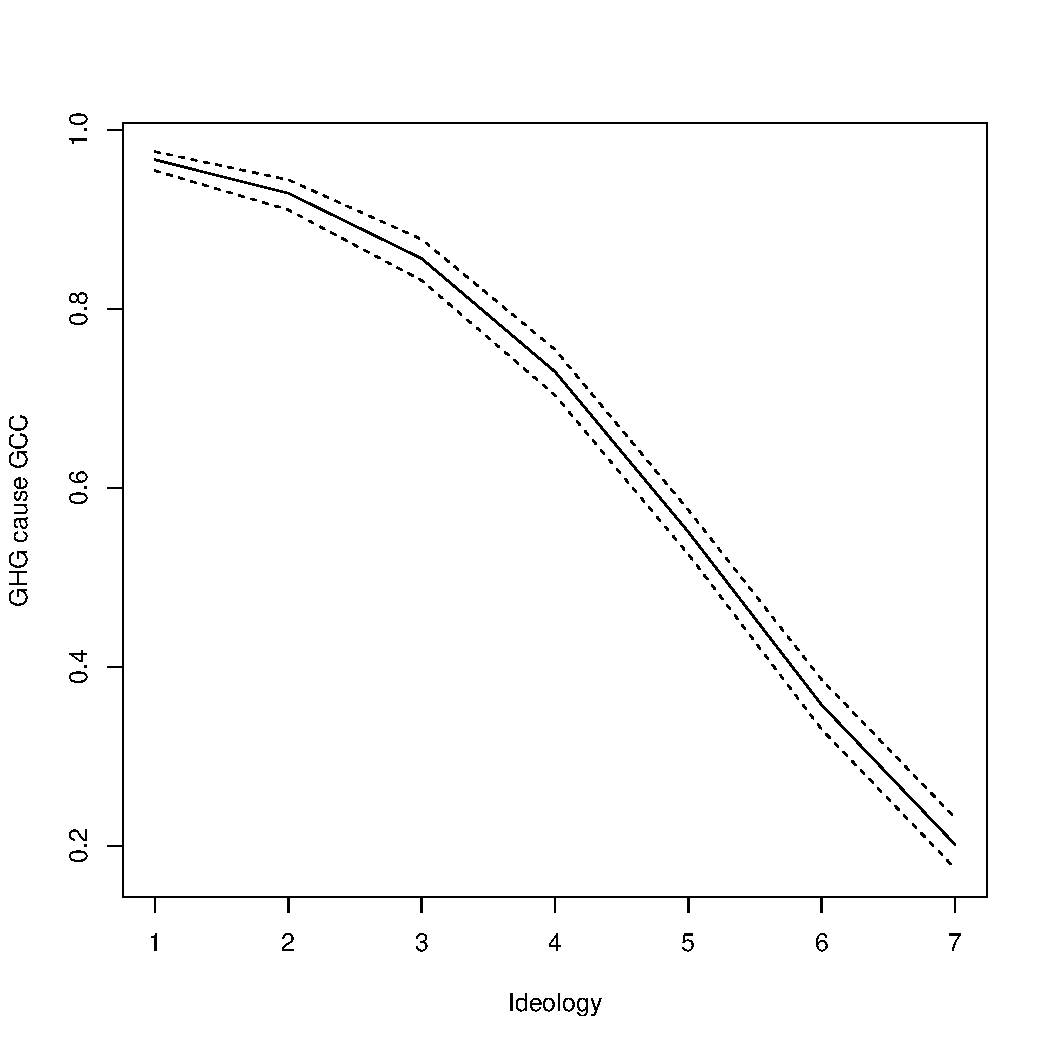
\includegraphics[width=4in]{../16_Logit/logitplot.pdf}%filename
        \caption{Predicted Probability of believing that Greenhouse
          Gases cause Climate Change by Ideology \label{fig:logitplot}}
\end{figure}   
			                  
\noindent We can see that as respondents become more conservative, the probability of believing that climate change is man-made decreases at what appears to be an increasing rate.   

\section{Summary}

As an analysis and research tool, logit modeling expands your capabilities beyond those that can reasonably be estimated with OLS. Now you can accommodate  models with binary dependent variables. Logit models are a family of generalized linear models that are useful for predicting the odds or probabilities, of outcomes for binary dependent variables. This chapter has described the manner in which logits are calculated, how model fit can be  characterized, and several methods for making the logit results readily interpretable.

Perhaps one of the greatest difficulties in applications of logit models is the clear communication of the meaning of the results. The estimated coefficients show the change in the log of the odds for a one unit increase in the $X$ variable -- not the usual way to describe effects. But, as described in this chapter, these estimated coefficients can be readily transformed into changes in the odds, or the logit itself can be ``reversed" to provide estimated probabilities.  Of particular utility are logit graphics, showing the estimated shift in $Y$ from values of zero to one; the estimated probabilities of $Y$=1 for cases with specified combinations of values in the $X$ variables; and estimates of the ranges of probabilities for $Y$=1 across the ranges of values in any $X$. 

In sum, the use of logit models will expand your ability to test hypotheses to include a range of outcomes that are binary in nature. Given that a great deal of the phenomena of interest in the policy and social sciences are of this kind, you will find this capability to be an important part of your research toolkit. 
\end{document}
